\subsection{重构定理}%
\label{sub:Reconstruction theorem}

回忆每个 CohFT 都定义了一个弗罗贝尼乌斯代数。若相应的弗罗贝尼乌斯代数是半单的，则我们称该 CohFT 为\textit{半单}的。

\begin{thm}[Teleman {\cite{Teleman2012}}]%
\label{thm:teleman}
    设 $\Omega$ 是一个具有平坦单位的半单 CohFT，$\omega$ 为其拓扑部分。则存在唯一的
    \[ R = \mr{Id} + R_1 z + \cdots \in \End(V)\ps{z} \]
    使得
    \[ \Omega = R.\omega. \]
\end{thm}

\begin{exm}
    回忆之前的霍奇丛 CohFT。回忆它由以下公式给出
    \[ \Omega^{\E}_{g,n} = c(\E) = 1 + \lambda_1 + \cdots + \lambda_g. \]
    取零次部分，我们看到 $\omega^{\E}$ 是点的 GW CohFT。利用 Mumford 的计算
    \[ \ch(\E) = g + \sum_{k=1}^{\infty} \frac{B_{2k}}{(2k)!}\ab(\kappa_{2k-1} + \frac{1}{2}\iota_*\sum_{i=0}^{2k-2} \bar{\psi}_1^{i} (-\bar{\psi}_2)^{2k-2-i}), \]
    其中 $\kappa_{m} = p_* \bar{\psi}_{n+1}^{m+1}$，$B_{2k}$ 是伯努利数，$\iota$ 是边界在 $2:1$ \'etale 覆盖意义下的嵌入，以及任意向量丛 $E$ 的公式
    \[ c(E) = \exp \ab(-\sum_k (-1)^k (k-1)!\ch_k(E)) \]
    （或者直接使用量子 Riemann-Roch 定理\footnote{Coates-Givental 中有一个符号错误，该错误已传播到其余文献中。}），我们得到 $R$-矩阵
    \[ R(z) = \exp\ab( \sum_{k=1}^{\infty} \frac{B_{2k}}{2k(2k-1)} z^{2k-1}) = 1+\frac{1}{12}z + \cdots. \]

    作为验算，我们将利用 $R$-矩阵计算 $\Omega_{1,1}^{\E}$。首先，我们考虑~\Cref{fig:03graphloop} 中的稳定图。
    \begin{figure}[htpb]
    \begin{center}
    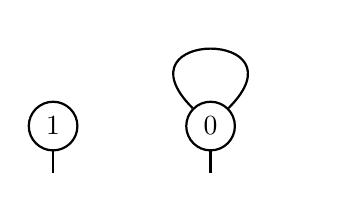
\begin{tikzpicture}[scale=1, transform shape, every loop/.style={}]
    \node[circle,draw=black,thick] (B) at (-1,0) {$1$};
    \draw[-,thick] (B) -- (-1,-0.6);
    \node[circle,draw=black,thick] (A) at (1,0) {$0$};
    \draw[-,thick] (A) -- (1,-0.6);
    \path[every node/.style={font=\sffamily\small},thick]
        (A)   edge[loop] (A);
    \end{tikzpicture}
    \end{center}
    \caption{稳定图，$g=1, n=1$}%
    \label{fig:03graphloop}
    \end{figure}
    第一个图 $\Gamma_1$ 给出贡献
    \begin{align*}
        \Cont_{\Gamma_1} &= T\omega_{1,1}^{\E}(R(z)^{-1}\1) \\
        &= \omega_{1,1}^{\E}(R(z)^{-1}\1) + p_* \omega_{1,1}^{\E}(R(z)^{-1}\1, T_R(z)).
    \end{align*}
    利用公式 $B_2 = \frac{1}{6}$ 以及 $\dim \Mbar_{1,1} = 1$ 这一事实，这变为
    \[ 1 - \frac{1}{12}\psi_1 + \frac{1}{12} \kappa_1. \]
    第二个图没有尾贡献，因为 $\dim \Mbar_{0,3} = 0$。边贡献的常数项为 $\frac{1}{12}$，故考虑自同构并前推到 $\Mbar_{1,1}$，得到
    \[ \Cont_{\Gamma_2} = \frac{1}{12} \Delta, \]
    其中 $\Delta$ 表示边界除子（带有正确的叠结构）。因为此时 $\psi_1 = \kappa_1$，我们得到
    \[ 1+\lambda_1 = 1 + \frac{1}{12}(\kappa_1 - \psi_1 + \Delta) = 1 + \frac{1}{12} \Delta. \]
\end{exm}




\subsection{算符形式与几何量子化}%
\label{sub:Operator formalism and geometric quantization}

我们将回到 Givental 的辛形式体系。这对某些计算更方便，但它实际上与我们之前的内容相同，至少在我们想要计算生成函数时是如此。回忆我们在 $V$ 上有弗罗贝尼乌斯流形结构，并考虑了带有辛形式
\[ (\mbf{f}(z), \mbf{g}(z)) \coloneqq \on{Res}_{z=0} \eta(\mbf{f}(-z), \mbf{g}(z)). \]
的向量空间 $\mc{V}\coloneqq V\ls{z^{-1}}$。若我们考虑由 $\mc{V}_+ = V[z]$ 与 $\mc{V}_- = z^{-1}V\ps{z^{-1}}$ 给出的极化，则令 $\bq$ 如之前（带有膨胀子平移）那样，设 $\bp$ 为 $\mc{V}_-$ 上的坐标，使得 $(\bq, \bp)$ 构成 $\mc{V}$ 的一组达布坐标。

\begin{defn}
    我们将形如
    \[ \mc{D} = \exp\ab(\sum_{g=0}^{\infty} \hbar^{g-1} \mc{F}_g) \]
    的任何形式函数称为\textit{福克空间的渐近元}。
\end{defn}

于是给定福克空间的这样一个渐近元，我们按以下公式对 $\mc{V}$ 上的（无穷小）辛变换进行量子化：
\[ \wh{p_a p_b} \coloneqq \hbar \partial_{q_a} \partial_{q_b}, \qquad \wh{p_a q_b} \coloneqq q_b \partial_{q_a}, \qquad \wh{q_a q_b} = \frac{q_a q_b}{\hbar}. \]
特别地，这将使我们能够理解像 $\hat{R} \mc{D}$ 这样的表达式。然而，我们需要小心，因为我们的公式将同时涉及基本解 $S_{\tau}$ 与 $R$-矩阵，而 $S_{\tau}$ 是 $z^{-1}$ 的幂级数。\footnote{这是因为我展开 $\frac{1}{z-\psi} = \sum_{n=0}^{\infty} \psi^n z^{-n-1}$。}

\begin{thm}[Givental {\cite{Givental2001quantization}}]
    形如 $S(z^{-1}) = \mr{Id} + S_1 z^{-1} + \cdots$ 的算符按以下公式作用于福克空间的（渐近）元
    \[ \hat{S}^{-1} \mc{D}(\bq) = e^{\frac{1}{2\hbar}W(\bq,\bq)} \mc{D}([S \bq]_+), \]
    其中 $W = \sum \eta(W_{mn}q_m, q_n)$ 由以下公式定义
    \[ \frac{S(w^{-1})^* S(z^{-1}) - \mr{Id}}{w^{-1}+z^{-1}} = \sum \frac{W_{mn}}{w^m z^n}. \]
    形如 $R(z) = \mr{Id} + R_1 z + \cdots$ 的算符按以下公式作用
    \[ \hat{R}\mc{D}(\bq) = e^{\frac{\hbar}{2} V(\partial_{\bq}, \partial_{\bq})} \mc{D}(R^{-1} \bq), \]
    其中 $V = \sum \eta(p_m, V_{mn} p_n)$ 由下式定义
    \[ \frac{R(w)^* R(z) - \mr{Id}}{w+z} = \sum V_{mn} w^m z^n. \]
\end{thm}

对于半单 CohFT，存在一组\textit{典范坐标} $u_{\alpha}$，使得 $1$-形式 $\d{u}$ 是代数同态 $T_v V \to \C$。于是在半单点附近，量子联络存在形如
\[ \Psi \cdot  R \cdot e^{\frac{U}{z}}, \]
的渐近解，其中 $\Psi$ 将平坦坐标变换为典范坐标，$U = \on{diag}(u_{\alpha})$ 是典范坐标的矩阵。最后，定义
\[ C = \frac{1}{2} \int^u \sum R_1^{\alpha\alpha} \d{u_{\alpha}}. \]
Teleman 重构定理的一个推论是公式
\[ \mc{D}^X = e^{C(u)} \hat{S}^{-1}_{\tau} \hat{\Psi} \hat{R} \wh{e^{\frac{U}{z}}} \prod_{i=1}^{\dim V} \mc{D}^{\mr{pt}} \]
它对任何具有半单量子上同调的光滑射影簇的格罗莫夫-威滕理论成立。

\begin{exm}
    作为最后一个例子，我们将应用 Teleman 定理计算任意半单 CohFT 的 $F_1$。设 $e_{\mu}$ 表示量子积的幂等基。我们将计算
    \[ \int_{\Mbar_{1,1}} \Omega_{1,1}(e_{\beta}). \]
    利用重构定理，我们得到
    \begin{align*}
        \int_{\Mbar_{1,1}}\Omega_{1,1}(e_{\beta}) ={}& \int_{\Mbar_{1,1}} T_R \omega_{1,1}(R(\bar{\psi})^{-1} e_{\beta}) + \frac{1}{2} T_R \omega_{0,3}(R(\bar{\psi})^{-1} e_{\beta}, V(\bar{\psi}_2, \bar{\psi}_3)) \\
        ={}& \int_{\Mbar_{1,1}}T_R\omega_{1,1}(e_{\beta}) - \int_{\Mbar_{1,1}} T_R \omega_{1,1}(R_1 e_{\beta})\bar{\psi} \\ 
        &+ \frac{1}{2}\sum_{\mu}  \omega_{0,3}(e_{\beta}, R_1 e^{\mu}, e_{\mu}) \\
        ={}& \int_{\Mbar_{1,1}} ( \omega_{1,1}(e_{\beta}) + p_* ( \omega_{1,2}(e_{\beta}, R_1 \1) \bar{\psi}_2^2 )) \\
        &- \int_{\Mbar_{1,1}} (\omega_{1,1}(R_1 e_{\beta})\bar{\psi}_1 + p_* ( \omega_{1,2}(R_1 e_{\beta}) \bar{\psi}_2^2 ) \bar{\psi}_1) \\
        &+ \frac{1}{2} \sum_{\mu} \eta(e_{\beta} \star e_{\mu}, R_1 e^{\mu}) \\
        ={}& \frac{1}{24} \sum_{\mu} ( \omega_{0,4}(e_{\mu}, e^{\mu}, e_{\beta}, R_1 \1) -\omega_{0,3}(e_{\mu}, e^{\mu}, R_1 e_{\beta}) )\\
        &+ \frac{1}{2} \eta(e_{\beta}, R_1 e^{\beta}) \\
        ={}& \frac{1}{24} \sum_{\mu}\sum_{\nu} \omega_{0,3}(e_{\mu}, e^{\mu}, e_{\nu})\omega_{0,3}(e^{\nu}, e_{\beta}, R_1 \1) \\
        &-\frac{1}{24} \sum_{\mu} \omega_{0,3}(e_{\mu}, e^{\mu}, R_1 e_{\beta}) + \frac{1}{2} (R_1)_{\beta\beta} \\
        ={}& \frac{1}{24} \ab(\eta(e^{\beta}, R_1 \1) - \sum_{\mu} \eta(e^{\mu}, R_1 e_{\beta})) + \frac{1}{2} (R_1)_{\beta\beta}.
    \end{align*}
    利用恒等式
    \begin{align*}
        \eta(R_1 \1, e^{\beta}) - \sum_{\mu} \eta(R_1 e_{\beta}, e^{\mu}) &= \sum_{\mu} \Delta_{\mu} \int_{\Mbar_{0,4}} \Omega_{0,4}(e_{\mu}, e_{\mu}, e_{\mu}, e_{\beta}) \\
        &= -\frac{1}{2}\sum_{\mu} \Delta_{\mu} \partial_{u_{\beta}} \Delta_{\mu}^{-1} \\
        &= \frac{1}{2} \sum_{\mu} \partial_{u_{\beta}} \log \Delta_{\mu},
    \end{align*}
    其中 $\Delta_{\mu} \coloneqq \eta(e_{\mu}, e_{\mu})^{-1}$，我们得到结果
    \[ \int_{\Mbar_{1,1}} \Omega_{1,1}(e_{\beta}) = \frac{1}{48} \sum_{\mu} \partial_{u_{\beta}} \log \Delta_{\mu} + \frac{1}{2} (R_1)_{\beta\beta}, \]
    它可写成如下具有启发性的形式
    \[ \d{F_1^{\Omega}} = \sum_{\mu} \ab( \frac{\d{\log \Delta_{\mu}}}{48} + \frac{1}{2} (R_1)_{\mu\mu} \d{u_{\mu}} ). \]
    这恢复了 Givental 已知的一个结果。
\end{exm}

\subsection{如何计算 R-矩阵}%
\label{sub:How to compute the R-matrix}

最后，我们将解释如何计算 R-矩阵，从弗罗贝尼乌斯流形是共形的这一情形开始（例如光滑射影簇的格罗莫夫-威滕理论、\(r\)-spin 曲线等）。在这个例子中，我们按照~\cite{PPZ2015} 考虑 3-spin 曲线的弗罗贝尼乌斯流形。设 \(V\) 是 2 维的，坐标为 \(x\) 与 \(y\)，其中 \(x\) 对应单位。度量为
\[ \eta = \begin{pmatrix}
    0 & 1 \\
    1 & 0
\end{pmatrix} \]
初级亏格零势为 \(F(x,y) = \frac{1}{2} x^2 y + \frac{1}{72} y^4\)。存在一个\textit{欧拉向量场}
\[ E = x \pdv{}{x} + \frac{2}{3} y \pdv{}{y}, \]
它分别以权 \(-1\) 与 \(-\frac{2}{3}\) 作用于 \(\partial_x\) 与 \(\partial_y\)。共形维数为 \(\delta = \frac{1}{3}\)，我们将定义次数算符
\[ \mu(v) = [E,v] + \ab(1 - \frac{\delta}{2})v. \]
这里，\(\partial_x\) 的次数为 \(-\frac{1}{6}\)，\(\partial_y\) 的次数为 \(\frac{1}{6}\)。

为方便起见，我们设 \(\phi = \frac{y}{3}\)，并定义
\[ \hat{\partial}_x = \phi^{1/4} \partial_x, \qquad \hat{\partial}_y = \phi^{-1/4} \partial_y, \]
然后在此框架下计算。在此设定下，量子乘法由下式给出
\[ \hat{\partial}_x \star \hat{\partial}_x = \phi^{1/4} \hat{\partial}_x, \qquad \hat{\partial}_x \star \hat{\partial}_y = \phi^{1/4} \hat{\partial}_y, \qquad \hat{\partial}_y \star \hat{\partial}_y = \phi^{1/4} \hat{\partial}_x. \]
我们所需的最后一点是，由 \(E\) 给出的量子乘法为
\[ E \star - = \begin{pmatrix}
    x & 2 \phi^{3/2} \\
    2 \phi^{3/2} & x 
\end{pmatrix}. \]
我们现在利用递推方程
\[ [R_{k+1}, E \star -] = (k + \mu) R_k. \]
计算 \(R\)-矩阵 \(R = 1 + R_1 z + \cdots\)。设 \(R_k = \begin{psmallmatrix}
    a_k & b_k \\
    c_k & d_k
\end{psmallmatrix}\)，我们得到方程
\[ \ab[
    \begin{pmatrix}
        a_{k+1} & b_{k+1} \\
        c_{k+1} & d_{k+1}
    \end{pmatrix}, \begin{pmatrix}
        x & 2 \phi^{3/2} \\
        2 \phi^{3/2} & x 
    \end{pmatrix}
] = \frac{1}{6} \pdiagmat[empty={}]{6k-1, 6k+1} \begin{pmatrix}
    a_k & b_k \\
    c_k & d_k 
\end{pmatrix}. \]

它的唯一解实际上是
\begin{align*}
    a_k &= \frac{1}{1728^k \phi^{3k/2}} \frac{1+6k}{1-6k} \frac{(6k)!}{(3k)!(2k)!} \delta_{k, \text{even}},  \\
    b_k &= \frac{1}{1728^k \phi^{3k/2}} \frac{1+6k}{1-6k}\frac{(6k)!}{(3k)!(2k)!} \delta_{k, \text{odd}},  \\
    c_k &= \frac{1}{1728^k \phi^{3k/2}}\frac{(6k)!}{(3k)!(2k)!} \delta_{k, \text{odd}}, \\
    d_k &= \frac{1}{1728^k \phi^{3k/2}} \frac{(6k)!}{(3k)!(2k)!} \delta_{k, \text{even}}. 
\end{align*}
如果你熟悉曲线模空间上的重言关系，你会看到级数 \(a_k + b_k\) 与 \(c_k + d_k\) 出现在 Faber-Zagier 关系的表述以及 Pixton 关系的表述中。

在弗罗贝尼乌斯流形不是共形的情形（例如等变格罗莫夫-威滕理论），我们需要使用振荡积分或其他某种技巧来确定 R-矩阵中的初值。我们在这里给出一个例子计算，它归功于 Givental~\cite{Givental2001semisimple}。在此设定下，\(X = \P^n\)，但该论证可适用于任何 Fano 环面簇。回忆 \(\P^n\) 的等变镜像为超势
\[ W = x_1 + \cdots + x_{n+1} + \sum_{i=1}^{n+1} \lambda_i \log x_i \]
（这里，为方便起见我们改变等变参数的符号）。因此，振荡积分将形如
\[ I = \int_{\Gamma \subset E_q = (x_1 \cdots x_{n+1}=q)} e^{W/z} \prod_{i=1}^{n+1} \frac{\d{x_i}}{x_i}. \]
它被算符
\[ \prod_{i=1}^{n+1}\ab(zq \odv{}{q} -\lambda_i) - q, \]
湮灭，这正是射影空间的 I-函数所满足的 Picard-Fuchs 方程。

为了在临界点附近展开此积分，我们首先需要计算临界点。这里，利用坐标 \(t = \log q\) 与 \(T_i = \log x_i\)，我们得到方程
\[ x_i = L - \lambda_i, \]
其中 \(L\) 是拉格朗日乘子。它们满足方程
\[ \prod_{i=1}^{n+1} (L - \lambda_i) = q, \]
因此对于一般的 \(\lambda\) 值，在 \(q = 0\) 附近，拉格朗日乘子的可能取值 \(L_i\) 由它们从哪个 \(\lambda_i\) 开始而区分。注意到函数 \(W\)、拉格朗日乘子的取值，从而临界点，都连续依赖于 \(\lambda\)，故当 \(q \neq 0\) 时它们在 \(\lambda = 0\) 处有非等变极限。

当 \(q = 0\) 时，矩阵 \(\Psi\) 从平坦基 \(\ab{H^i}\) 过渡到基
\[ L_i(H) = \prod_{j \neq i} \frac{H - \lambda_j}{(\lambda_i - \lambda_j)^{1/2}}, \]
它们是典范坐标的首项（只需通过等变局部化计算环面作用的不动点，我们便会得到这个拉格朗日插值）。因此，我们需要在 \(q = 0\) 极限下计算 \(L_j \ab(z q \odv{}{q}) I\)。直接计算表明，将 \(L_i \ab(z q \odv{}{q})\) 作用于积分会给振荡积分的被积函数引入一个与 \(\frac{q}{x_i}\) 成正比的额外因子。因为我们可以置换指标，我们只计算 \(i = n+1\) 的情形。另一次直接计算表明，除非 \(j = n+1\)，否则积分在 \(q = 0\) 处为零，故实际上我们看到 \(R\) 在经典极限下是对角的。当 \(j = n+1\) 时，我们有
\[ \frac{q}{x_{n+1}} = x_1 \cdots x_n, \]
积分变为
\[ \int_{\Gamma} e^{\ab( \sum_{i=1}^n x_i + (\lambda_i - \lambda_{n+1})\log x_i ) / z} \d{x_1} \cdots \d{x_n} = \prod_{i=1}^n \int_{\R} e^{x_i/z} x_i^{(\lambda_i - \lambda_{n+1})/z} \d{x_i}, \]
它只是伽马函数的乘积。

\begin{lem}
    我们有以下渐近展开
    \[ \log \Gamma(1+s) \sim s \log \ab(\frac{s}{e}) + \frac{1}{2} \log(2\pi s) + \sum_{k=1}^{\infty} \frac{B_{2k}}{2k} \frac{s^{1-2k}}{2k-1}. \]
\end{lem}
利用它，我们看到在 \(q = 0\) 处，R-矩阵的对角矩阵元为
\[ \log R = \sum_{k=1}^{\infty} \frac{B_{2k}}{2k} \frac{z^{2k-1}}{2k-1} \sum_{i =1}^n (\lambda_i - \lambda_{n+1})^{1-2k}. \]
根据 Givental 的一个结果，这意味着此 R-矩阵恢复了 \(\P^n\) 的等变 GW 理论；作为推论，由于非等变极限存在，我们得到 \(\P^n\) 的 Virasoro 约束。
